\documentclass{beamer}
 
\usepackage[utf8]{inputenc}
\usepackage[english]{babel}
\usepackage{amsmath}
\usepackage{amsfonts}
\usepackage{amssymb}
\usepackage{graphicx} 
\usepackage{latexsym} 
\usepackage{listings}
\usepackage{xcolor}
\usepackage{soul}
\usepackage[T1]{fontenc}
\usepackage{amsthm}
\usepackage{mathtools}
\usepackage{setspace}
\usepackage{array,multirow,makecell}
\usepackage{geometry}
\usepackage{textcomp}
\usepackage{float}
\usepackage{bbold}
\usepackage{wrapfig}
\usepackage{textpos}

\rmfamily

\usetheme{Madrid}
%%\usecolortheme{beaver}



\title{LP 16 Facteur de Boltzmann}
\author{Naïmo Davier}
\institute{Université Paul sabatier}

 
\begin{document}
	
\begin{frame}
	\titlepage
\end{frame}

\addtocounter{framenumber}{-1}
\title{Facteur de Boltzmann}

\begin{frame}
\frametitle{Atmosphère isotherme}
\centerline{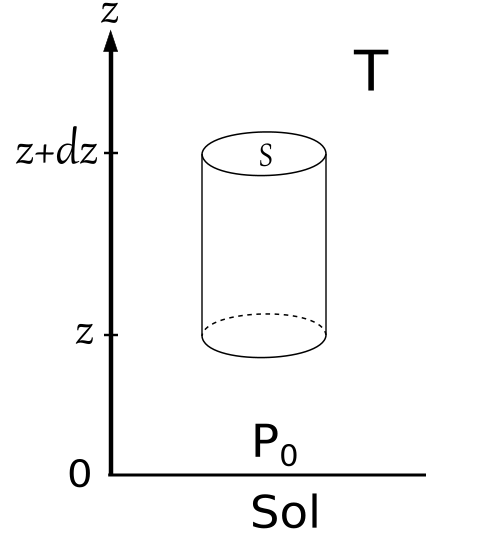
\includegraphics[width=6.5cm]{atm_iso}}
\end{frame}

\begin{frame}
\frametitle{Compétition entre densité d'état et facteur de Boltzmann}
\centerline{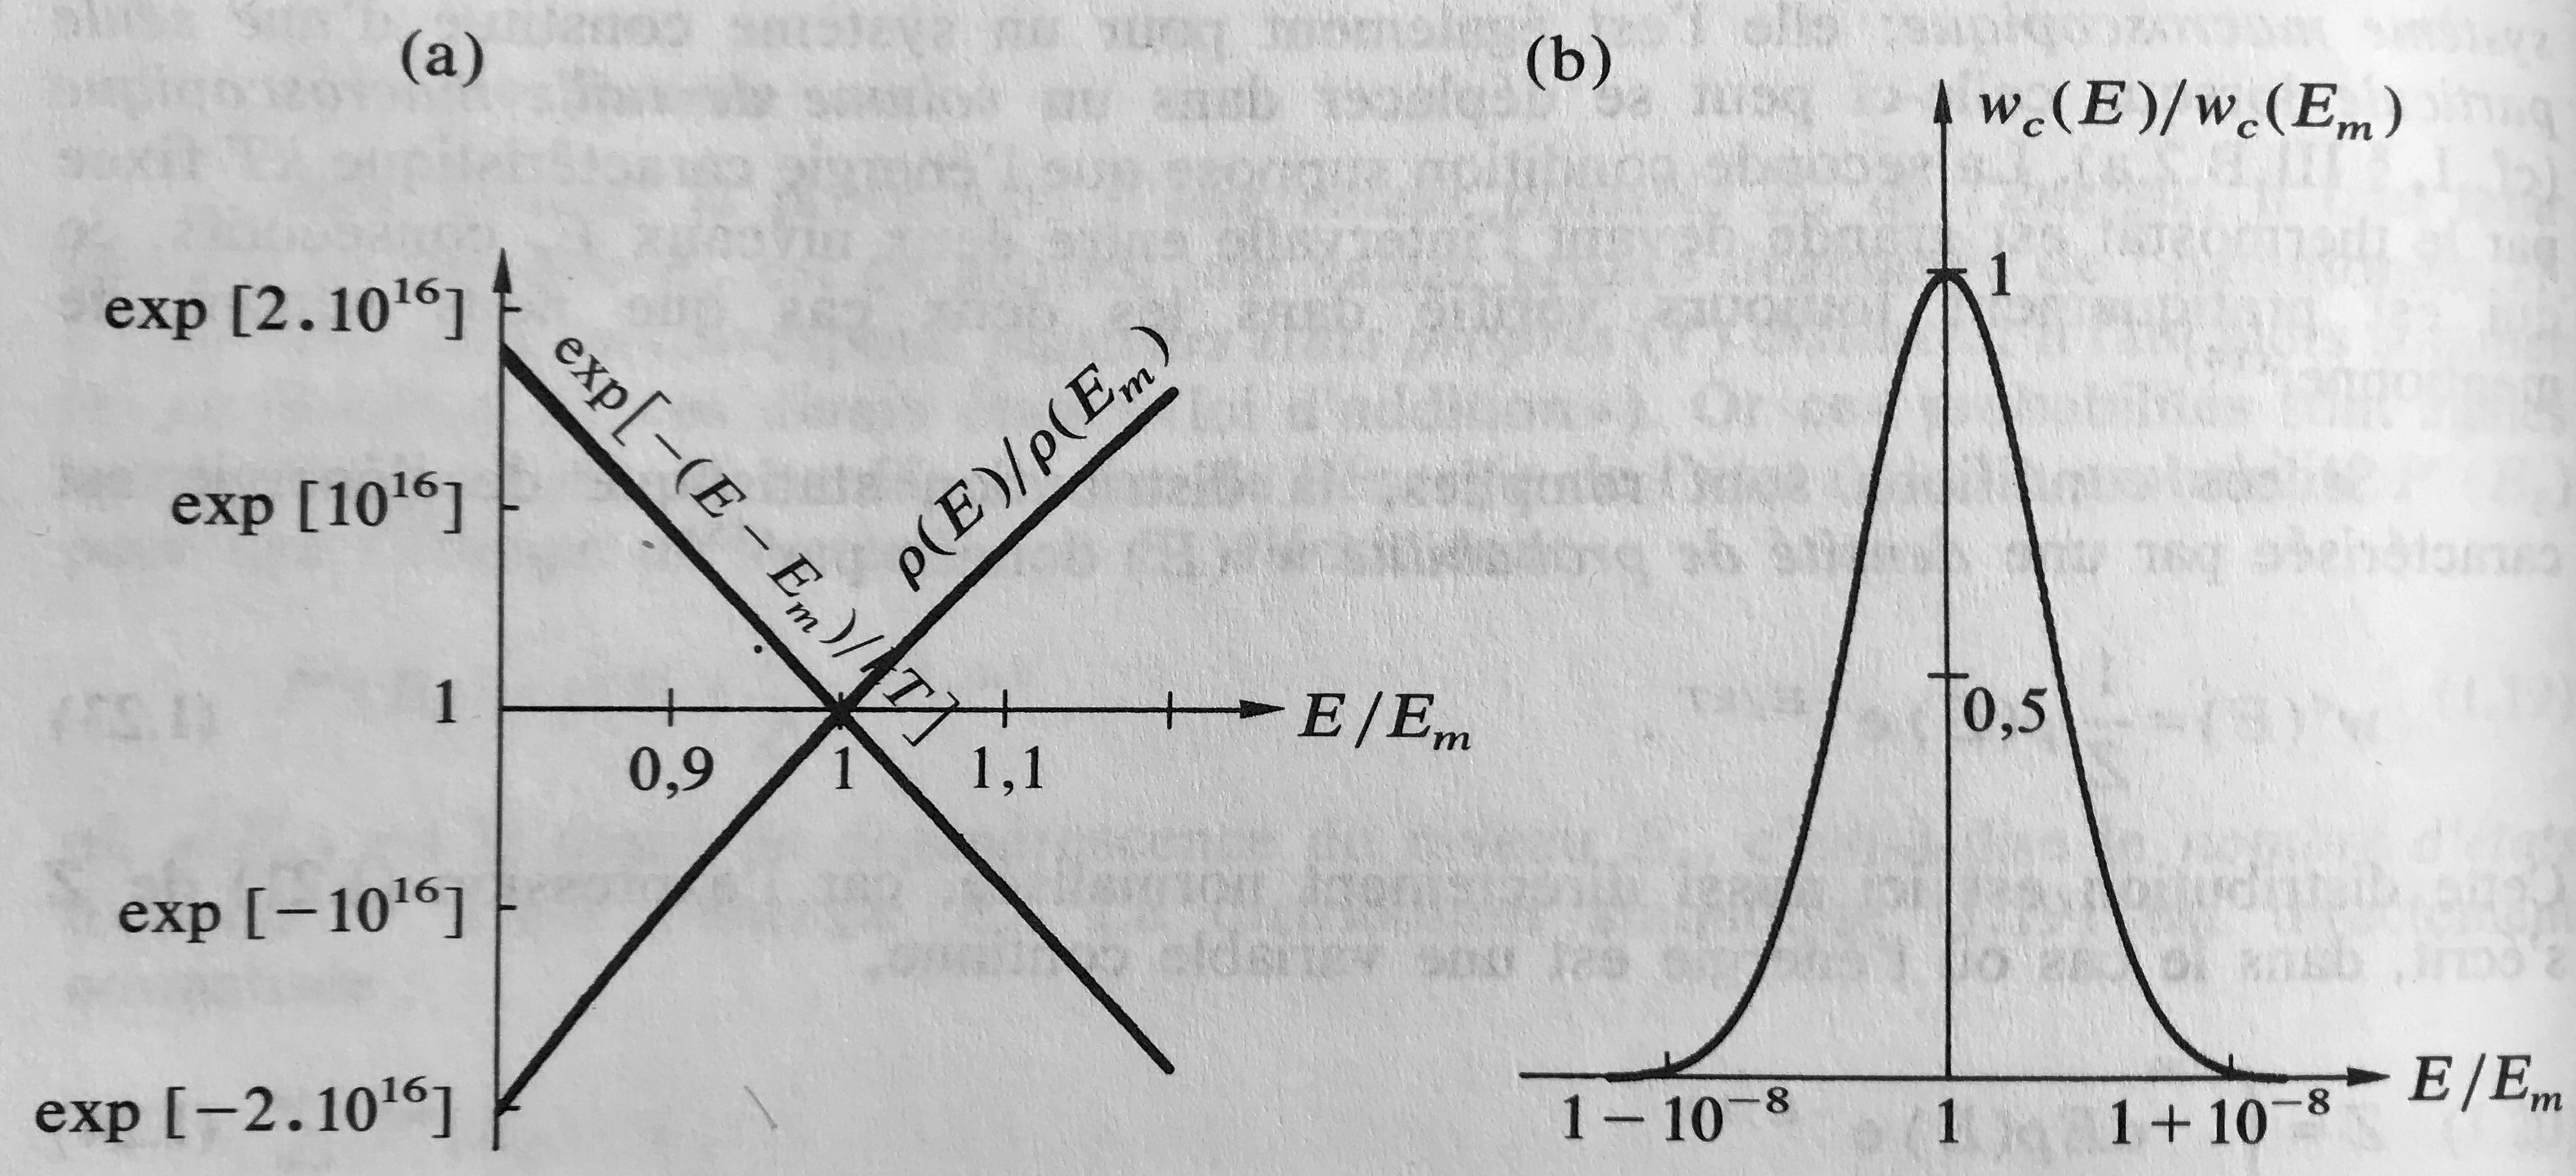
\includegraphics[width=12cm]{competition}}
\end{frame}

\begin{frame}
\frametitle{Capacité calorifique, formulaire}
Pour le calcul de $\bar{E}$, on a
\begin{eqnarray}
\frac{\partial }{\partial \beta}\ln(\mathrm{sinh}\, \alpha \beta) = \alpha \frac{\mathrm{cosh}\, \alpha \beta}{\mathrm{sinh}\alpha \beta} = \alpha\, \mathrm{coth}\, \alpha \beta
\end{eqnarray}
Pour le calcul de $C_V$, on a
\begin{eqnarray}
\frac{\partial }{\partial \beta} \mathrm{coth}\, \alpha \beta = \frac{\partial }{\partial \beta} \frac{\mathrm{cosh}\, \alpha \beta}{\mathrm{sinh}\, \alpha \beta} =  \alpha \frac{\mathrm{sinh}^2\alpha \beta - \mathrm{cosh}^2\alpha \beta}{\mathrm{sh}^2\alpha \beta}
\end{eqnarray}
or on sait que $\;\mathrm{cosh}^2\alpha \beta - \mathrm{sinh}^2\alpha \beta =1$
\begin{eqnarray}
\Longrightarrow \frac{\partial }{\partial \beta} \mathrm{coth}\, \alpha \beta = -\alpha \frac{1}{\mathrm{sinh}^2\alpha \beta}
\end{eqnarray}
Finalement 
\begin{eqnarray}
\frac{\partial }{\partial T} \mathrm{coth}\, \alpha \beta =   \frac{\partial \beta}{\partial T} \frac{\partial }{\partial \beta} \mathrm{coth}\, \alpha \beta = \frac{1}{k_BT^2} \alpha \frac{1}{\mathrm{sinh}^2\alpha /k_BT}
\end{eqnarray}
\end{frame}

\begin{frame}
\frametitle{Capacité calorifique}
\centerline{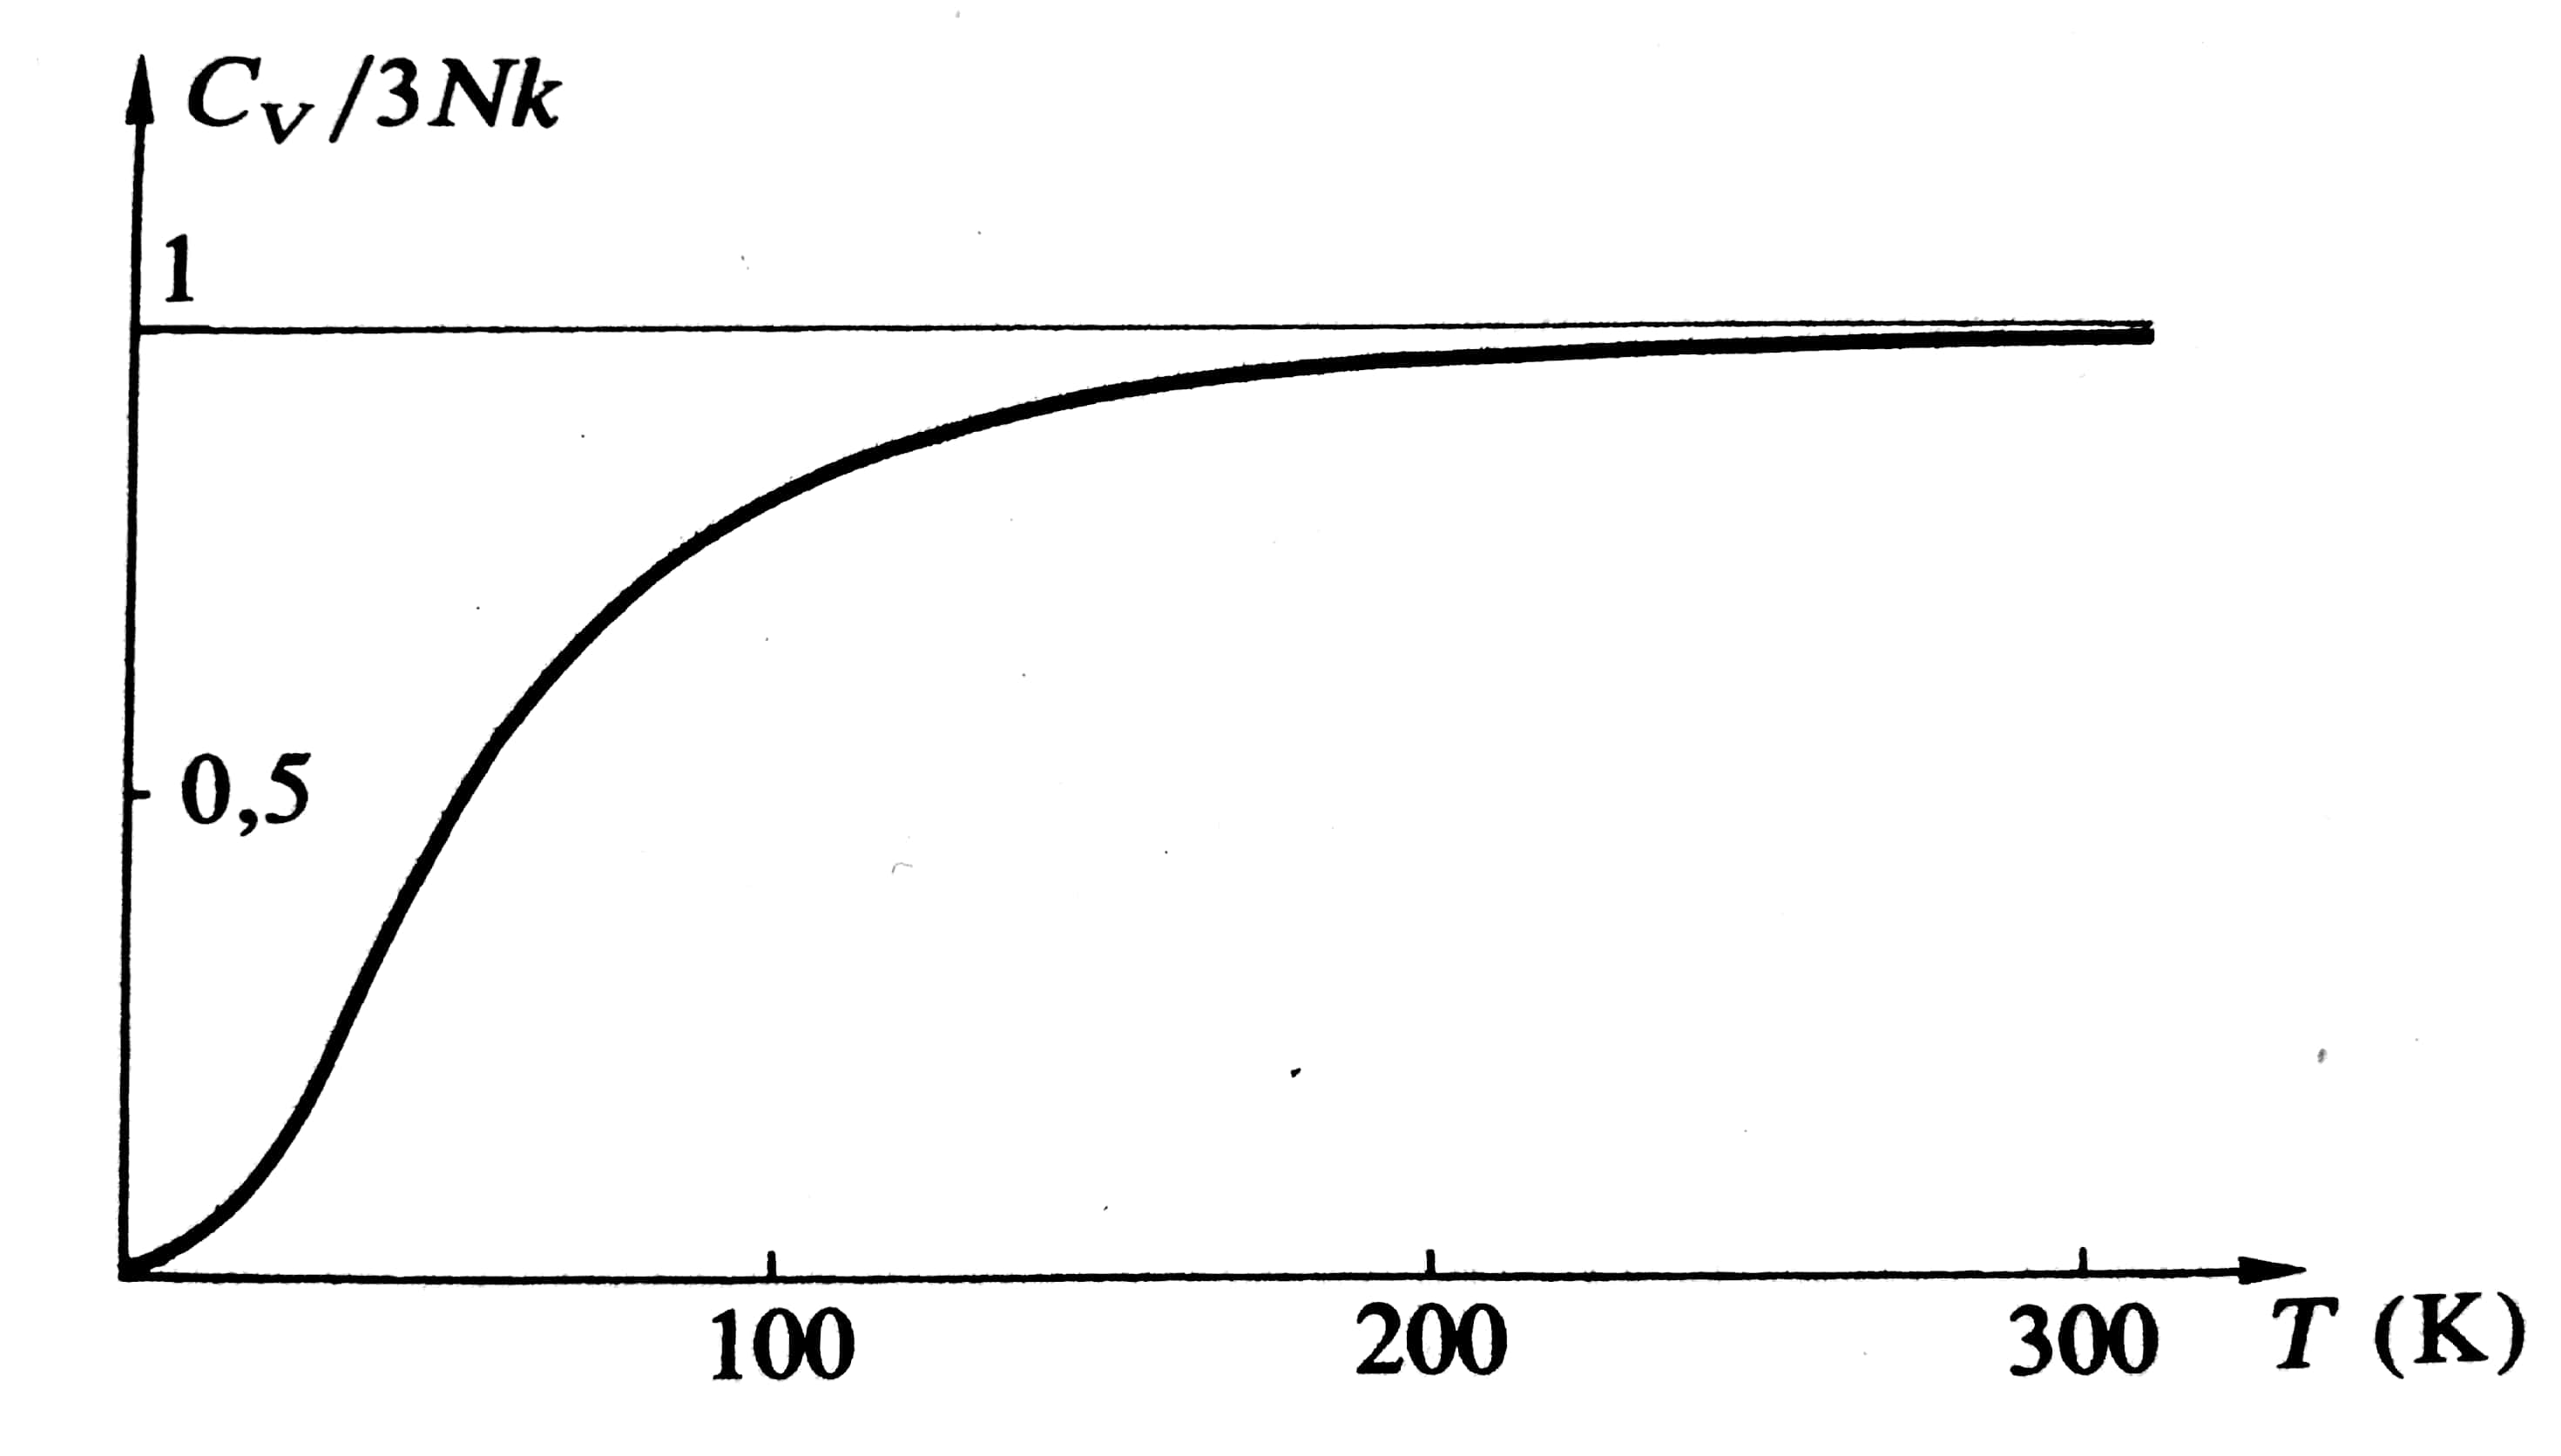
\includegraphics[width=11cm]{C_V}}
\end{frame}

\end{document}